\chapter{Methodology of Refactoring Process}
\label{chapter:methodology}
In addition to the theoretic contributions made in the previous chapter, the primary aim of the following work is to provide a more comprehensive view on refactoring with a direct application to our case. In this chapter it will be argued that refactoring should be placed in a much broader context, as it directly relates to multiple software domains, such as code smell detection, testing, and measuring quality improvements. Including these domains, Figure \ref{fig:extended-model} portrays a resulting \emph{refactoring process}. It depicts refactoring as a sequence of connected stages, and thereby furthers our current understanding. In addition, both business related sections of previous chapter \ref{sec:Business} are incorporated in this process, indicating the stages they influence.

\bigskip % Adds empty line
\begin{figure}[htp]
    \centering
    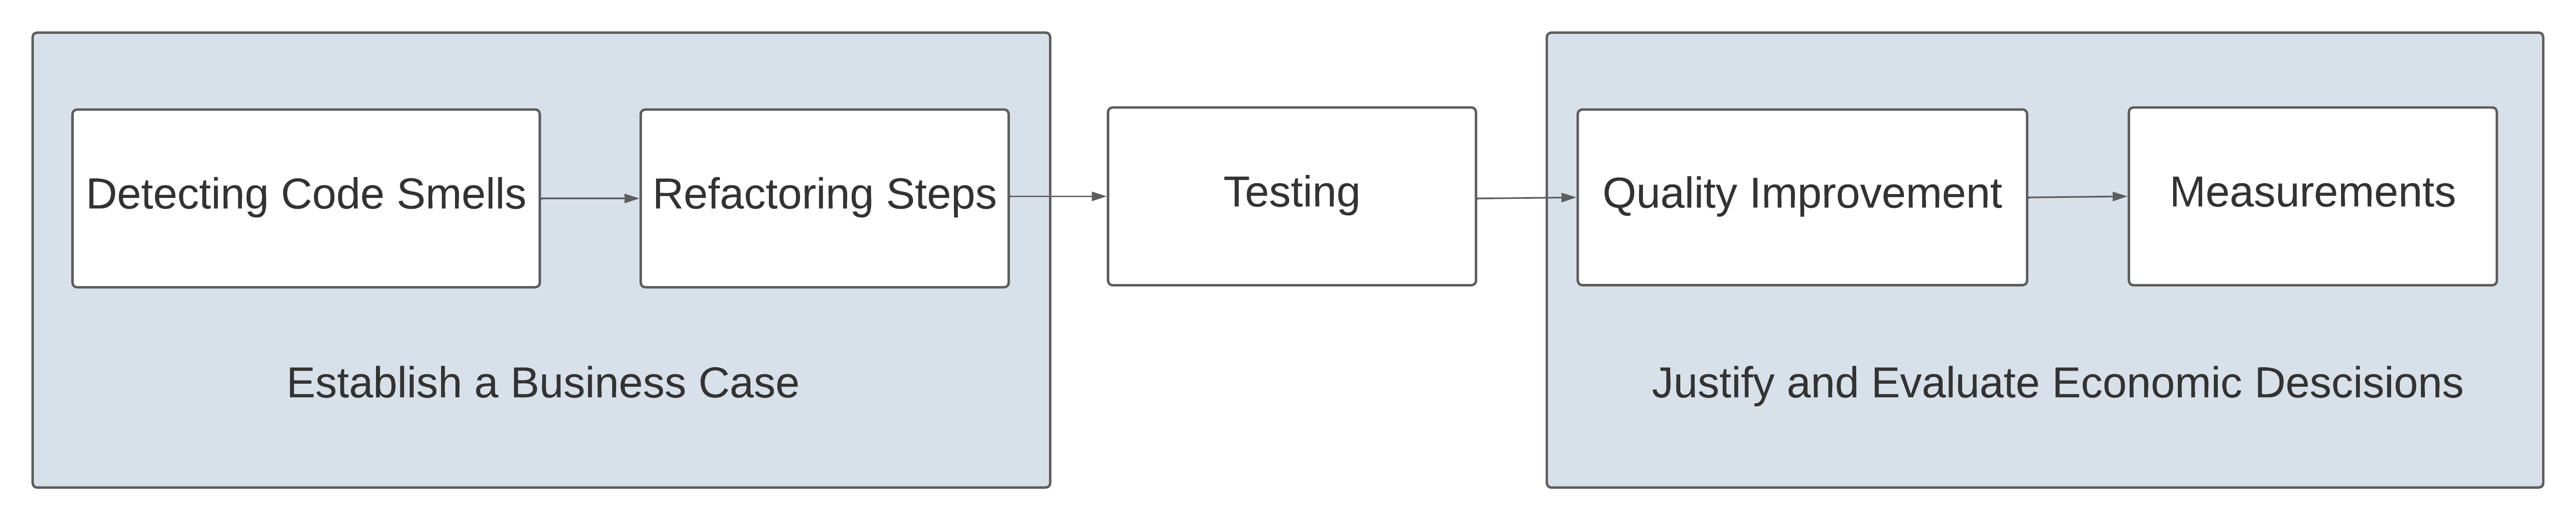
\includegraphics[width=\textwidth]{./assets/extended_refactoring}
    \caption{Refactoring process (Extended Model)}
    \label{fig:extended-model}
\end{figure}
\bigskip % Adds empty line

\section{Detecting Code Smells}

% Catalogue
As stated before, not all 24 code smells listed by Martin Fowler. Instead, the 10 most frequently reported code smells have been chosen according to the study of conducted by \textcite{lacerda2020}.
Further, two additional smells \emph{refused bequest} and \emph{data clumps} were discarded. The decision was made due to their focus on inheritance and data structures, respectively. These two programming abstractions are not utilized in the software system, and are thus not relevant in the detection. In order to revisit the code smell catalog with their corresponding explanation, refer to Table \ref{fig:smells}. 


Two primary reasons exist that have led to the decision of restricting the amount of smells for this section. First, it is not in the scope of the thesis to find every single code smell of the software system. Instead, the aim is to find the problems that are most apparent. Second, including more smells would be less of a problem, if automatic code detection tools could be used. Without having automatic detection, limiting the amount of smells is reasonable. A detection approach based on automatic tools is unfortunately not available for the python programming language, as will be alluded to in the following section.

\subsection{Detection Methods}
% Metrics based
Many tools have been created to automatically or semi-automatically detect code smells (\cite{menshawy2021}). In the context of our thesis, the code smells are detected semi-automatically using a metrics-based approach. This approach measures source code elements and takes decisions based on threshold values (\cite{menshawy2021}). It fulfills two important requirements necessary for the following work. On the one hand, it contains automation to a certain extent, increasing the efficiency and standardization compared to manual approaches. Further, it can be used for the python programming language, which is an essential prerequisite for the software system at hand. Menshawy additionally points out that a metrics-based approach does not provide metrics for every code smells. Nevertheless, for the eight smells relevant for the thesis, an appropriate metric was found (see Table \ref{fig:metrics}). 

% Automation based
Using a detection approach utilizing automated tools would have been more attractive, but unfortunately not possible.  It is the most used approach (\cite{menshawy2021}), but availability strongly depends on the programming language the software system is written in (\cite{menshawy2021}). Further, looking at Menshawy's research on the most cited tools, it can be observed that a significant difference exists between the java programming language, which was supported  by 48\% of the tools and python, which was supported by mere 4\%. In addition, by researching possible automated tools appropriate for python, it was evident that at this moment of time, the offering is insufficient to accomplish a comprehensive detection strategy. 

% Manual approach
In the beginning, the author also considered following a manual approach. In contrast to automation, the manual detection relies on human perception of smells by applying predefined guidelines (\cite{menshawy2021}). It is characterized as highly time-consuming and prone to human error. Therefore, when comparing this approach to a metrics-based, it is less desirable and was subsequently discarded as a detection technique.

% Visualization
Another detection approach that has not yet been mentioned, is the detection by means of code visualization. Although it can only detect a small subset of the code smells, visualization supported the detection of code smells by including a dependency graph (see figure \ref{fig:pre-refactor}).

\subsection{Sonargraph}
% Intro Sonargraph
The detection of code smells relied heavily on a code analyzer tool called \emph{Sonargraph}. Its usage proved to be extremely useful in the detection of code smells, by its ability to compute and list metrics of the software system. The software included a diverse selection of metrics. These metrics provided insights to find problems regarding the entire project and its individual modules. For each metric, Sonargraph offered explanations, which allowed for an appropriate metric to be found for each relevant code smell.

% Explorer + Metrics
Compared to other software solutions, Sonargraph was chosen for several reasons. Although the full suite of Sonargraph Applications is not free of charge, its graphical application \emph{Sonargraph Explorer} was free to use. For the thesis, it provided both numerical and visual methods to make observations about the code base. All the tools needed to compute metrics were accessible. Another noteworthy benefit of using Sonargraph during the detection, was its ability to observe the entire project,  and not just at individual files. For instance, this was essential for metrics inspecting the dependencies between modules. In addition, it was beneficial not having to rely on a multitude of software tools, by having just one software solution.

% Code duplicate
It is important to note that there was no appropriate metric that could detect code duplication. However, in its paid version, accessible within a trial period, an automatic tool to detect code duplicates was provided.  Previously, it was stated that it was difficult to find automatic tools to detect code smells in a software system written in python. Duplicate code particularly differs from the other smells, as it can be detected independent of the programming language. To detect duplications of code in programs, the software does not need to understand the syntax. This same mechanism could theoretically detect duplications in other types of text that are not programs. 

\subsection{Metrics Overview}

\begin{table}[htp]
    \centering
    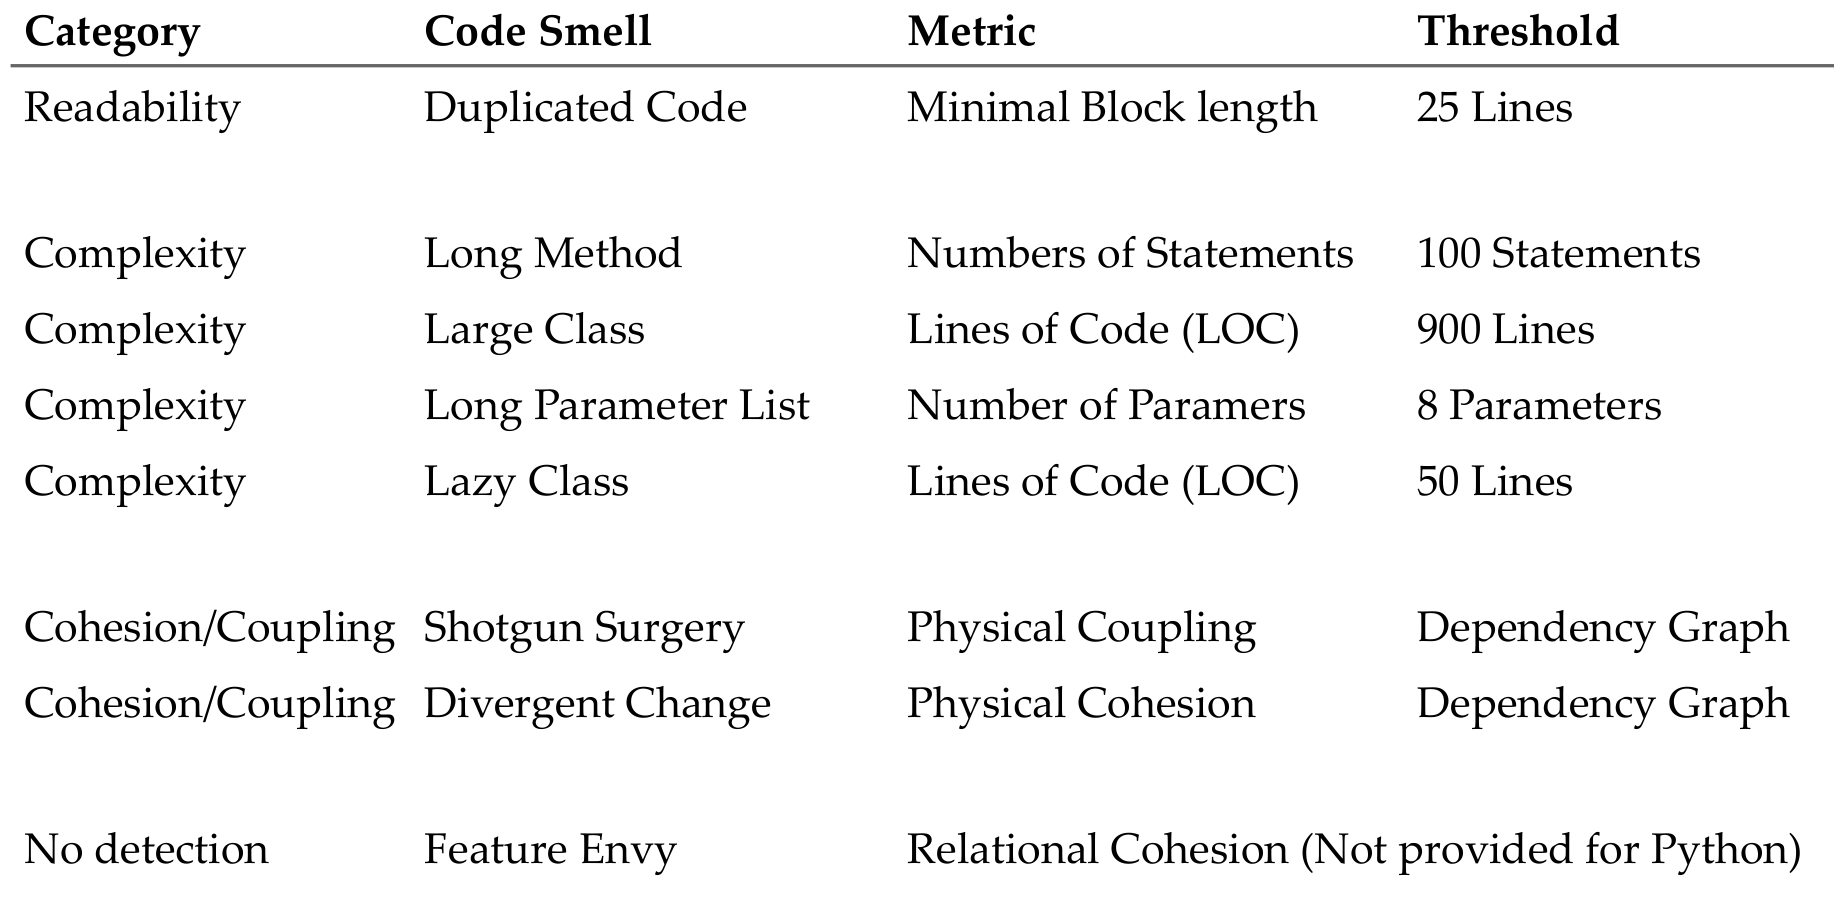
\includegraphics[width=\textwidth]{./assets/smell_overview}
    \label{fig:metrics}
    \caption{Metrics Overview}
\end{table}

% Table
Table \ref{fig:metrics} presents the corresponding metric for each code smell. In addition, for certain metrics, a threshold value is given. When the threshold value is surpassed, there is an indication that this code smell exists in the software system.

% Subgroups
Individual metrics are categorized into three subgroups, named after the quality attribute they best represent. More importantly, however, this distinction is made, as each of the group differs in terms of the detection approach. For example, as mentioned before, the subgroup readability differs considerably due to the fact that code duplication is automatically detected. In this case, the application limits the detection to a minimum of 25 Lines. Meaning that only code duplicates are shown if they surpass this amount. 

% Complexity -> Threshold
Code smells in the subgroup named complexity, follow a typical metrics-based approach. The threshold values indicate when a code smell is potentially present. Notably, all the metrics in this category involve counting of some sorts. Particularly, the smells are detected by counting the number of statements, lines of codes, and numbers of parameters of methods. Prioritization of given smells can be done by comparing the extent of how much a given threshold value is surpassed. Similarly, code smells can be discarded if the associated metric does not surpass the threshold value. 

% Cohesion/Coupling -> Dependency graph
Lastly, Shotgun Surgery, Feature Envy and Divergent change respectively are bound to the coupling and cohesion of the software system. We use the metric \emph{Physical cohesion} for both Feature envy and Divergent change, and \emph{Physical coupling} for Shotgun Surgery. \emph{Relational cohesion}, which would better detect feature envy, is not provided for the python language. Consequently, we will use Physical cohesion for the detection as well. The metrics themselves measure the dependencies “to” and “from” other components, in either the same module (Cohesion) or in other modules (Coupling). The appropriate threshold value highly depends on the size of the software system. By adding code to the code base, we naturally increase the amount of expected dependencies. Therefore, in order to appropriately argue the findings, incorporating a dependency graph in addition to the metrics seemed necessary in order to evaluate the prominence of these two code smells (refer to \ref{sec:findings-smells}).

\section{Testing}
\label{sec:testing}
% Transition

\subsection{Importance of Testing in a Refactoring Process}

% Importance of Tests
Turning now to the importance of testing within the context of the refactoring process.  In order to understand the significance, it is appropriate to return to Martin Fowler's definition of refactoring (\cite{fowler2018}), as first discussed in section \ref{sec:background}. According to his definition, refactoring must not alter the external behavior of code. It was pointed out in the theoretical part of this thesis that by avoiding the changing of features, programmers can alleviate the risks associated with changing the codebase, which predominantly includes the introduction of new bugs. As a result, to demonstrate that the behavior of the code base was not altered during refactoring, testing is necessary. Therefore, without testing we would get a false sense of an improvement of code quality, as potentially negative alterations are not taken into consideration. Hence, only with testing we can ensure that after refactoring the software system is in a better state than before.

\subsection{Testing Cyber Physical Systems}
\label{sec:cps}

% CPS Hetereogenous Nature
Robots and other CPS react to information from the physical world and must operate safely even in the presence of uncertainties \cite{geissvolkermaria}. In such a dynamic real-world environment, \textcite{kapurpulkit2020} describes CPS testing, as a time-consuming and a particularly complicated task for programmers. He points out that this is due to the difficulty to ensure that a CPS will behave as expected. Furthermore, it is hard to define the boundaries and physical limitations of the testing landscape made for a CPS (\cite{abbaspourasadollah2015}). 

% Automation
Another limitation in CPS testing is the introduction of automated or semi-automated methods. Here, the feasibility of testing is limited to the hardware components of the CPS. For instance, a CPS with physical motions requires a considerable amount of time to run tests. Additionally, it potentially demands human supervision and manual intervention. Some of these challenges can be mitigated by using a physics-based simulation that mimics the real-world environment. (\cite{kapurpulkit2020}), also referred to as \emph{digital twin}. Such solutions do exists in practice, but are unfortunately unavailable to our software system. This challenging physical environment of CPS results in programmers having to satisfy multiple layers at the same time, when testing their software. The layers of CPS software testing contain verifying software, hardware, network, and the integration of all these components to work as a single system \cite{abbaspourasadollah2015}.

% Software test -> Manual test
In general, there is a high interest to use automated testing, as manual testing is more likely to produce errors {turlea2019}. Despite automated tests having multiple advantages, such as more testing in less time, it needs to be considered that no software tests are available for the software system at hand. In particular, the major disadvantages of automated tests are the costs associated with developing test automation, especially in a dynamic and customized environment (\cite{taipale2011}). Consequently, developing a testing suite from scratch forces us to choose a manual approach. It is important to note, that in future work, it would be appropriate to consider developing software tests. It is however not in the scope of this thesis to also take on this additional endeavor.

% One advantage
One characteristic of the physical nature of CPS is that we are able to make visual observations. This feature can be viewed as an advantage to advocate manual testing of a particular CPS. Whether the observation of a CPS can be used in testing, is arguably strongly dependent on the type of CPS. In our case, there are no restrictions in observing the system visually. The benefits of such an approach become especially apparent when taking into account that our software project is focussing on managing entire processes. In more concrete terms, we are able to perceive visual changes in the behavior of our CPS by running a predefined process.  

% Concluding thoughts
Overall, the lack of software tests and the ability to visually observe behavioral changes encouraged the decision to include manual testing,  as a preferred method. Even though test coverage is not thorough, this approach of testing can to some extent support that no alterations are present within a particular processes. As a result, it is an approach that suits the preconditions within our context, as it investigates changes within the scope of processes.

\subsection{Method selection}

% Transition
To reduce the inherent risks of uncertainty in manual testing, methods are selected based on their ability to test objectively and in a routinized manner. To achieve this goal, two methods have been chosen, where one enables testing automation, while the other improves objectivity. In particular, the software platform Camunda is used to automate the business processes and the domain specific language Gherkin is used to objectively formulate requirements. In combination, these tools deliver a procedure to reduce ambiguity, which is a fundamental prerequisite when trying to capture any cue in observable changes.

\begin{figure}[htp]
    \centering
    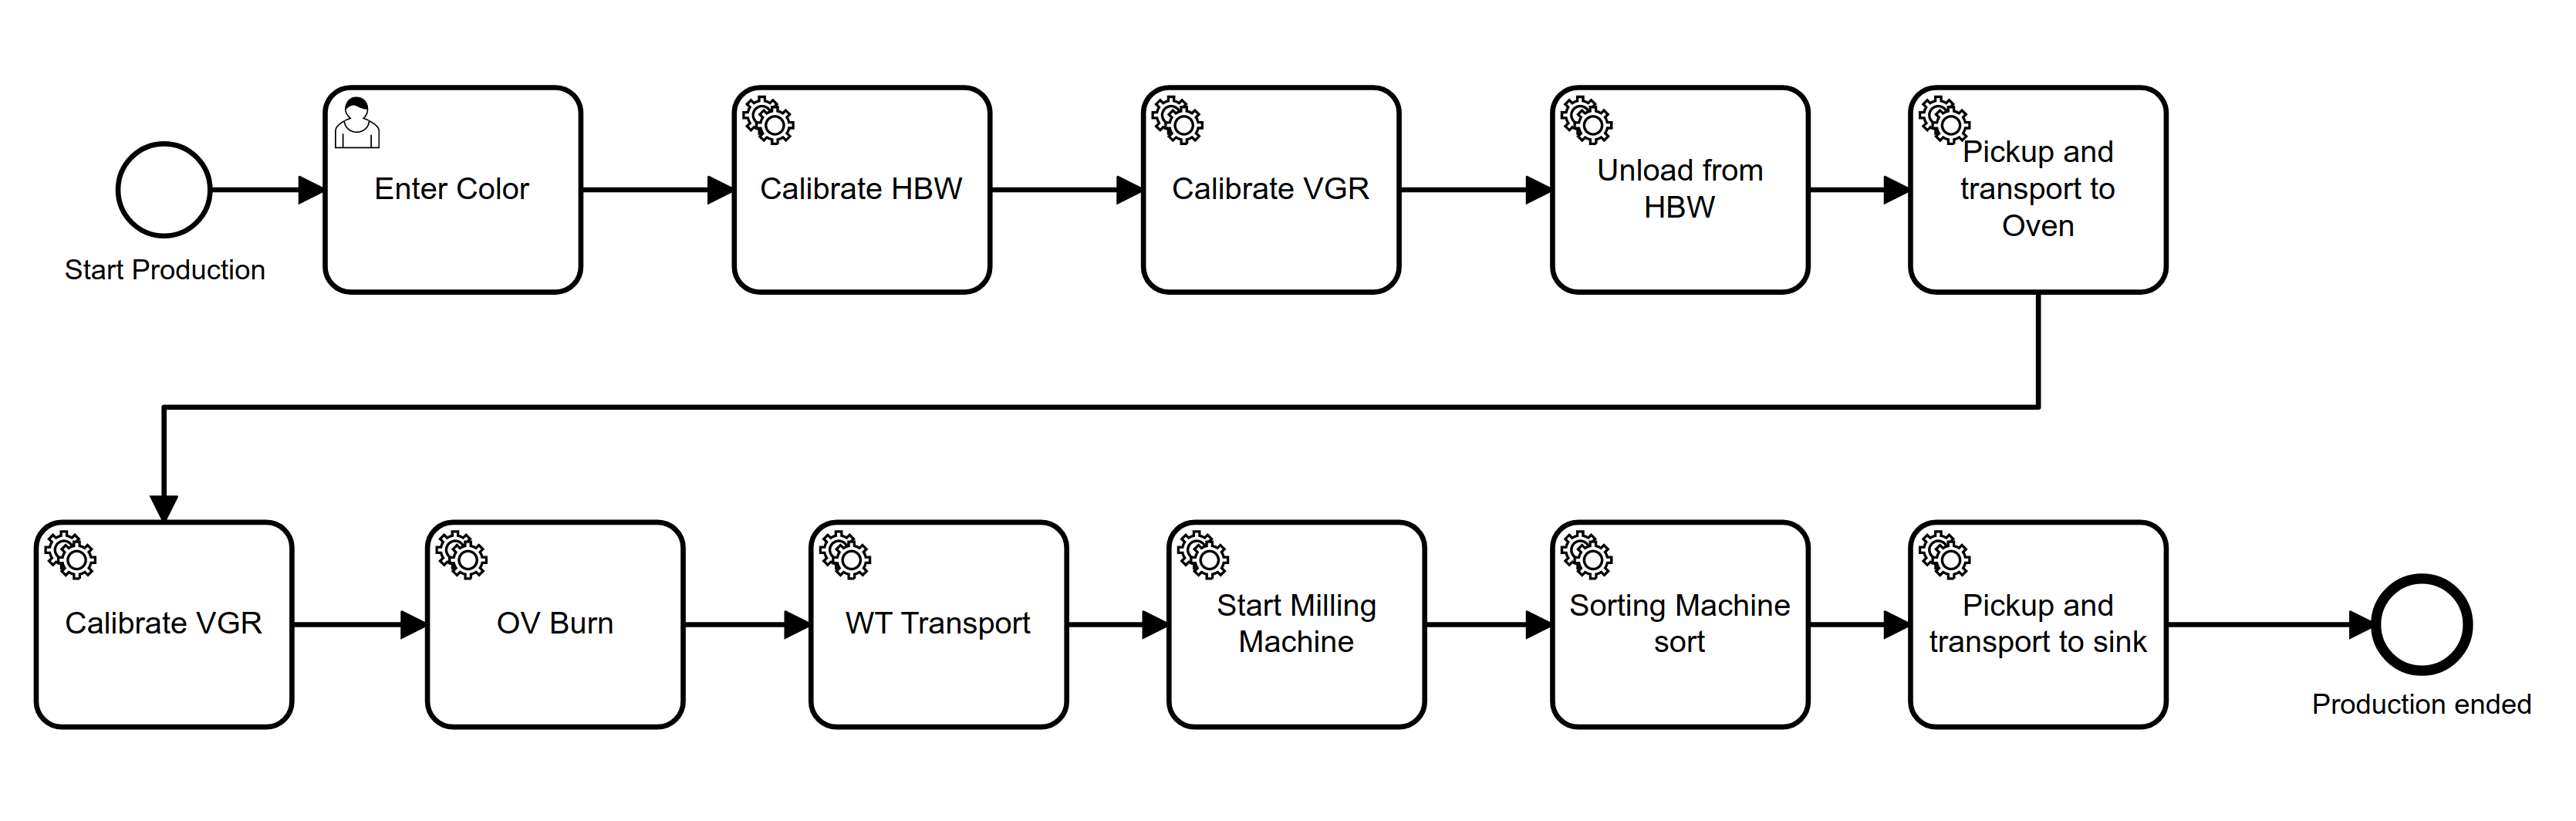
\includegraphics[width=\textwidth]{./assets/camunda_process}
    \caption{Camunda Production Process}
\end{figure}

% What we have
Even though there are no software tests available, multiple business processes, using the BPMN representation, have already been implemented for the present software system. These representations are stored in \emph{.bmpn} files and can be executed by the Camunda BPMN platform, which allows the automation of the these processes. For the testing, the production process has been chosen to best reflect the software system. Using this file, we are able to simulate an entire production process that includes all components of the factory. As a result, the testing can cover a major part of the software system's functionality. Using the contents of this file, the Camunda platform is able to sequentially do predetermined HTTP requests, which otherwise would have been done manually. Performing these requests manually would not only be very tedious, but also takes away standardization with a risk of making mistakes. In addition, the BPMN notation used by the Camunda platform allows us to visually inspect, which parts of the process are currently running. This is an exceptionally useful feature, when trying to find out where a current issue might be located, if the visual tests fail.


% Gherkin Explanation
Gherkin on the other hand is not a software application. Instead, it is a domain specific language that is generally used in conjunction with software. Hereby, one can formulate behavior in the form of specifications written in plain text, which is understandable by both humans and computers (\cite{zotero-undefineda}). It uses a set of special keywords that enables formulating these specifications in a structured way. We can then validate whether the software does what the specifications say. This validation is primarily done with corresponding software tools. However, in our case this will be done manually. Overall, this allows us to objectively test whether the software system fulfills these specifications, that can be routinely repeated in a standardized way. Refer to \ref{appendix:gherkin} to view an illustrative example in which the Gherkin keywords are directly applied to the software system.

\section{Measuring Quality Improvement}
\subsection{Importance}

% Importance of tracking
Having incorporated testing in our refactoring model, we are now in a position to consider methods to measure code quality after refactoring. Measuring code quality improvements allows us to evaluate how successful refactoring was. In particular, we can measure the extent of improvement, by comparing the refactored software system with its state prior to the refactoring. Having these measurements, allows us to reflect on refactoring endeavors and therefore helps us in making future decisions related to refactoring. Moreover, if the metrics are sufficiently accurate, one could argue when to initiate and when to stop refactoring, by using them as indicators. However, measurements are not limited to the comparison of the initial and final state of a refactoring. Measurement results can be further expanded by periodically measuring code quality. For instance, this allows us to individually attribute the quality improvement in relation to refactoring specific code smells. 

% Index
One possible metric that allows for quantifiable measurements, is the maintainability index, which measures how maintainable the source code is. This measure would be suitable for our case, as it offers single-valued quantification of code quality, while also considering multiple aspects of code quality. A more detailed account of the index will be given in the following section.

\subsection{Maintainability Index}
or
% Introduction
To compute the maintainability index, the python package Radon was used. Apart from the maintainability index, this software tool is able to compute raw metrics (SLOC, comment lines, blank lines), Cyclomatic complexity and Halstead volume. These listed metrics are all interconnected, as the maintainability index include all of these in its computation. The documentation of the software Radon offers explanations of the index and its implementation. The following section makes extensive use of the documentation in order to provide an overview (\cite{zotero-undefinedc}). To begin, one should look at the components of the formula of this index to better understand what it wants to achieve.  


Original Formula:
\begin{equation}
\label{eq:original}
\mathrm{MI}=171-5.2 \ln \mathrm{V}-0.23 \mathrm{G}-16.2 \ln \mathrm{L}
\end{equation}

\begin{itemize}
\item V = Halstead Volume
\item G = Cyclomatic Complexity
\item L = Source Lines of Code (SLOC)
\end{itemize}

Derivative (used by Radon):

\begin{equation}
\label{eq:radon}
\mathrm{MI}=\max \left[0,100 \frac{171-5.2 \ln \mathrm{V}-0.23 \mathrm{G}-16.2 \ln \mathrm{L}+50 \sin (\sqrt{2.4 \mathrm{C}}))}{171}\right]
\end{equation}

\begin{itemize}
\item C = Percentage of commented lines
\end{itemize}


The original equation \ref{eq:original}is included, as it makes it easier to understand how the individual components contribute to the final result. The second formula, which is used by Radon, is a derivative of the original formula. It is preferred as it is able to measures the maintainability between a scale from 0 to 100. As a consequence, the computation is easier to understand, as values closer to 100 indicate better maintainability. The second difference is that this formula also takes into account the percentage of commented lines indicated by the variable \emph{C}. It diminishes the significance of SLOC, when the source code contains a lot of commented lines. Although not specifically mentioned in the documentation, this is presumably the reason Radon included this additional variable. 

\subsection{Methods used for taking measurements}

% Challenges
The act of taking measurements is also a design decision that was consciously carried out. At first, taking the measurements manually was considered as a suitable method. Still, after some consideration, it was evident that an automated approach is more appropriate. One of the reasons was that manually running the software tool after each change quickly becomes a tedious task. Considerable amount of time would be spent for something that an easily be automated. There would also be no clear indication on the right amount of measurements to take in a routinized way. By making too many measurements, not only a lot of time is required, but it would also be difficult to differentiate between the individual measurements. Conversely, by having too few measurements, there would not be sufficient information available to arrive at meaningful conclusions.

% Git hook
Regarding the timing of the measurements, it became clear that measuring after each commit in the git version control program would be a suitable approach. That way each measurement could directly be attributed to individual commits, which includes information on code changes (commit message) and the possibility to check the difference to the previous state of the program (diffs). 

Fortunately enough, there exists an intuitive way to run scripts in conjunction with git activities. These types of scripts are called \emph{git hooks} or simply \emph{hooks}. As a result a hook was written using the bash command language, implemented in a way that it is executed prior to each git commit. Consequently, this approach solved both concerns of time inefficiency and lack of attribution. It is important to note, however, that this was only possible due to Radon being a command line utility. If graphical software had been used, only a manual approach would have been feasible, if not directly implementable by the graphical software itself. 

% Features
The bash script performs two distinct functions: computing and saving. Initially, it executes radon to compute the maintainability index, including its subcomponents. Next, these computations are then saved by writing them to a file. This file is saved locally on the computer, named after the date and time of execution. This allows attribution of the measurements to each commit. What is special about this methodology is that it enables continuous tracking in three dimensions. First, we are able to attribute individual refactoring steps in the form of commits. Second, we are able to more broadly connect measurements to the refactoring of individual code smells, preferably by indicating smells in commit messages. Lastly, by comparing current measurements to the initial state of the project, we can evaluate the overall progress since starting the refactoring.